\documentclass[a4paper,12pt]{article}

\usepackage[utf8]{inputenc} % encodé en utf-8
\usepackage[T1]{fontenc} % compatible avec les accents

\usepackage[french]{babel} % rédigé en français
\usepackage[hyphens]{url} % formatte les liens en autorisant la césure au niveau des traits d'union
\usepackage[urlcolor=black,colorlinks=true,linkcolor=black,citecolor=black]{hyperref} % liens cliquables mais non colorés

\usepackage[top=25mm, bottom=25mm, left=35mm, right=25mm]{geometry} % définit les marges
\usepackage{array} % permet l'alignement vertical dans les tableaux
\usepackage{setspace} % permet de régler l'interligne
\onehalfspacing % définit l'interligne 1,5 par défaut

\usepackage{graphicx} % gestion des images
\graphicspath{ {../images/}}
\usepackage{array} % gestion des tableaux
\usepackage{csquotes} % gestion des guillemets

\usepackage{fourier} % utilise une autre police que celle par défaut (Computer Modern) fourier - venturis - libertine - tgtermes - kpfonts - lmodern - txfonts - newtxtext,newtxmath - mathptmx - stix 

\usepackage{fancyvrb}

\usepackage[backend = biber, style = authoryear, useprefix = true, maxbibnames = 99]{biblatex}


%\addbibresource{}

\DefineBibliographyExtras{french}{%
\protected\def\mkbibnamefamily#1{%
\textsc{\textnohyphenation{#1}}}
}%

\DefineBibliographyStrings{french}{%
    page  = {\lowercase{p.}}, % for single page number
    pages = {\lowercase{pp.}}, % for multiple page numbers
}

\DefineBibliographyExtras{french}{\renewcommand*{\bibrangedash}{\textendash}} % Pour rendre les "--" correctement

% \renewcommand*{\mkibid}{\emph} %ibid en italique  if authoryear-ibid

\usepackage{float}

\setcounter{secnumdepth}{3} %Ne compte pas plus loin que 1.1.1
\setcounter{tocdepth}{3}

\usepackage{enumitem} %% utilisé pour la présentation de fausse table des matières dans la table des matières commentée

\newlist{legal}{enumerate}{10}
\setlist[legal]{label*=\arabic*.}

\usepackage{ragged2e} % Permet de placer plus facilement les tableaux

\newcolumntype{R}[1]{>{\RaggedRight}p{#1}}

\title{Projet STIC-B505 : Budgetsquirrel, une application de gestion de budget} 
\author{Milena Albu \and Marie Huysman} % vos prénom et nom
\date{} % pas de date

%\usepackage{fancyhdr}
%\pagestyle{fancy} % Turn on the style
%\fancyhf{}
%\fancyhead[L]{\footnotesize \nouppercase \leftmark}
%\fancyhead[R]{\footnotesize \nouppercase \rightmark}
%\fancyfoot[C]{\thepage}
%
%\renewcommand{\chaptermark}[1]{%
%\markboth{#1}{}}
%
%    \renewcommand{\sectionmark}[1]{\markright{\thesection \ #1}{}}

\usepackage{longtable}


\begin{document} % début du corps du texte
\sloppy

\begin{titlepage} % style spécial pour la page de garde
\singlespacing % remet l'interligne normal pour cette page

%%alternative à la bannière image
%\begin{center} 
%\huge{\textsc{Université Libre de Bruxelles}}\\
%\vspace{.5cm}
%\LARGE{Faculté de Lettres, Traduction et Communication}
%\end{center}
%% Bannière image
\begin{figure}[h]
\noindent
\makebox[\textwidth]{
\includegraphics[scale=0.6]{banner.png}}
\end{figure}

\vfill % laisse LaTeX gérer l'espacement vertical

%VOIR SI LE TITRE CONVIENT

\begin{center}
\LARGE{Conception et gestion de banques de données : Rapport de projet}\\ % ajoutez votre titre ici
\Large{ Budget Squirrel : Application de gestion de budget}
\vspace{.5cm}
\end{center}

\vfill

\begin{tabular}{b{5.5cm}b{7.5cm}} % taille et alignement des cellules du tableau
 \\ Milena \textsc{Albu} \\ Marie \textsc{Huysman} \\ & Rapport de projet écrit dans le cadre du cours STIC-B505 : Conception et gestion de banques de données \\
\end{tabular}

\vfill

\begin{center}
Année académique 2020--2021 % vérifiez que l'année est correcte !
\end{center}

\end{titlepage}

\tableofcontents

\thispagestyle{plain}

\newpage

\section{Introduction}

%Si besoin de citer : \parencite[2--4]{SOURCE}
%Notes de bas de page \footnote{informations suppl.}

Dans le cadre de ce projet, nous avons choisi de développer une application appartenant au domaine de la gestion financière et permettant la gestion de budget à une échelle personnelle.
Le rapport ci-dessous en documente le processus de design et conception, ainsi que les développements successif et les améliorations apportées à l'idée de base décrite dans le rapport précédent.
Après une brève présentation du domaine d'application, nous présenterons notre schéma conceptuel, ainsi que sa traduction en schéma relationnel.
Ensuite, nous décrirons les différents éléments des scripts SQL que nous avons mis en place : clés uniques et étrangères, contraintes au niveau de la base des données, checks et triggers, ainsi que privilèges d'accès.
Par après, nous exposerons brièvement l'application Web que nous avons développée. 
Nous terminerons ce rapport en offrant quelques informations sur le développement du projet, ainsi qu'en exposant les conclusions que nous avons tirées lors de la finalisation de ce dernier.

En annexe à ce rapport, vous trouverez deux fichiers sql : \verb\initdb.sql\, qui contient le script permettant la création de la base de données en elle-même, et \verb\basicdata.sql\, qui peuple la base de données de quelques informations, permettant ainsi de parcourir les différentes pages de l'application ainsi que la base de données afin d'en comprendre leur fonctionnement. 
Toujours en annexe à ce rapport, nous avons joint les pages de notre application (9 en tout) : \verb\index.html\, \verb\inscription.php\, \verb\connexion.php\, \verb\homepage.php\, \verb\profil.php\, \verb\historique.php\, \verb\enregistrement.php\, \verb\stat.php\, et \verb\logout.php\. S'y trouvent également un dossier css contenant le boilerplate CSS Skeleton\footnote{\url{http://getskeleton.com/}}ainsi que les modifications que nous y avons apporté, un dossier img contenant les images utilisées dans l'application, et un fichier \verb\utils.js\ contenant une fonction JavaScript de redirection de page.

\textbf{NOTE : pour le zip final à rendre, ne pas inclure le readme, ni le dossier du rapport latex.}

\subsection{Domaine d'application}

Une application de gestion de budget est une application qui permet, au minimum, l'enregistrement ainsi que la suppression des transactions dans une base des données, la gestion des utilisateurs et de leur budget, et la possibilité d'agréger une vue d'ensemble sur les transactions financières enregistrés.
Afin de mettre en œuvre une telle application, les développeurs doivent connaître les besoins minimaux des utilisateurs potentiels, ainsi que les différentes techniques de programmation à employer pour répondre de manière pertinente, voir optimale, à ces besoins.
Dans le cas de Budget Squirrel, l'application se focalise sur les utilisateurs qui n’ont pas nécessairement une expertise spécifique avec le planning financier, mais qui souhaitent néanmoins avoir une vue d’ensemble, ainsi qu’un suivi quotidien, de leurs dépenses.
L'application est à usage restreint et, dans sa version actuelle (en usage libre, lié aux profils de ses utilisateurs, mais sans être protégée par un système de mot de passe) nous recommandons qu'elle soit employée au sein d'une réseau domestique, et sur un serveur local.

Comme convenu dans le rapport précédent, l'application sait gérer plusieurs cas d'utilisation: connexion et déconnexion, création et modification de profil, enregistrement et suppression des transactions, vue historique propre à chaque utilisateur, et accessible en mode consultation ainsi qu'en mode édition (permet la suppression des transactions listées), et vue statistique avec visualisation dynamique des données liées aux transactions par mois (graphique en barres), et par catégorie (diagramme circulaire).

L'application Budget Squirrel compte 9 écrans, divisés en 4 catégories:
\begin{enumerate}
\item gestion de profil (écran d’accueil index.html, page d'accueil de l'application, connexion, inscription, profil, et log out);
\item enregistrement (écran d'enregistrement de transaction);
\item historique des transactions (écran historique), et 
\item statistiques (écran statistiques).
\end{enumerate}

Dans la réalisation d'écrans, des éléments de PHP (76.2 \%), CSS (6.4 \%), HTML (1.9 \%),  et JavaScript (0.1\%) ont été utilisés. Le rapport, quant a lui, a été rédigé en utilisant LaTeX (15.4 \% de notre projet).

\newpage

\section{Schéma conceptuel}

Le schéma conceptuel de la base des données Budget Squirrel reste conforme au schéma validé lors de la première étape du projet. Nous comptons 5 tables principales, ainsi que 3 tables issues de la matérialisation de l’héritage sur la table transaction financière.

Concernant les attributs (mieux détaillés dans la section 3), chaque table en contient au minimum un identifiant (clé primaire), ainsi que des contraintes (clé étrangère, ou bien contraintes d'unicité, selon les besoins).

Nous avons appliqué quelques corrections par rapport au schéma conceptuel de notre premier rapport. La structure générale reste très proche de celle de notre premier schéma, mais nous avons apporté des modifications aux tables catégorie\_ tf, virement, budget\_ mensuel, et carte, soit pour nous conformer aux corrections demandées après la remise du premier rapport, soit après discussion lors d'une des guidances, lorsque nous nous sommes rendues compte que certains de nos éléments rajoutaient une complexité inutile à l'utilisation de l'application.

La table carte est devenue une entité faible, car nous considérons qu'une carte ne peut pas être identifiée seulement par son numéro, mais par la combinaison entre son numéro et le NISS de l'utilisateur. De plus, pour permettre une \og suppression \fg des cartes par l'utilisateur (ou plutôt une désactivation), nous avons ajouté un attribut permettant de définir le statut (activé ou non) de la carte. Enfin, pour ne pas afficher le numéro de la carte à travers l'application, nous avons ajouté un attribut de nom, qui permet à l'utilisateur de nommer sa carte. 

Nous avons aussi ajouté un élément de description à la table catégorie, ce qui permet de mieux comprendre chaque élément de la table, autant dans la base de données que du côté de l'application.

Des contraintes concernant les dates ont également été ajoutées, car il n'est pas possible qu'une date de transaction (et par conséquent, le mois et l'année d'un budget) précède la date de naissance de l'utilisateur qui l'a créée.

Une communication n'étant pas obligatoire lors d'un virement, nous considérons dans cette nouvelle version du schéma que le l'attribut communication de la table virement est un attribut facultatif.

Enfin, en cours de développement, nous avons fait le choix de supprimer les contraintes de reste et de clôture de chaque budget mensuel, car cela pouvait poser des problèmes de calcul : si le budget du mois de février est clos avant celui de janvier, et que son reste est ajouté au mois de mars, par exemple, à la clôture du budget du mois de janvier, il est difficile d'ajouter le reste au mois de février, et de répercuter le changement sur le mois de mars (et ainsi de suite).
Ainsi, pour proposer une application plus flexible, nous avons fait le choix de simplifier la table budget\_ mensuel et son fonctionnement, en supprimant les attributs de reste et de statut.
La clôture d'un budget n'est donc pas possible.
Cette suppression reste mineure, car l'application se concentre principalement sur la gestion du budget et des différentes transactions, que se soit de manière rétrospective, ou de manière prédictive. L'objectif principal reste atteint, et la gestion des différents budget n'en est que plus souple pour l'utilisateur.\\

\begin{figure}[!ht]
\noindent
\makebox[\textwidth][c]{
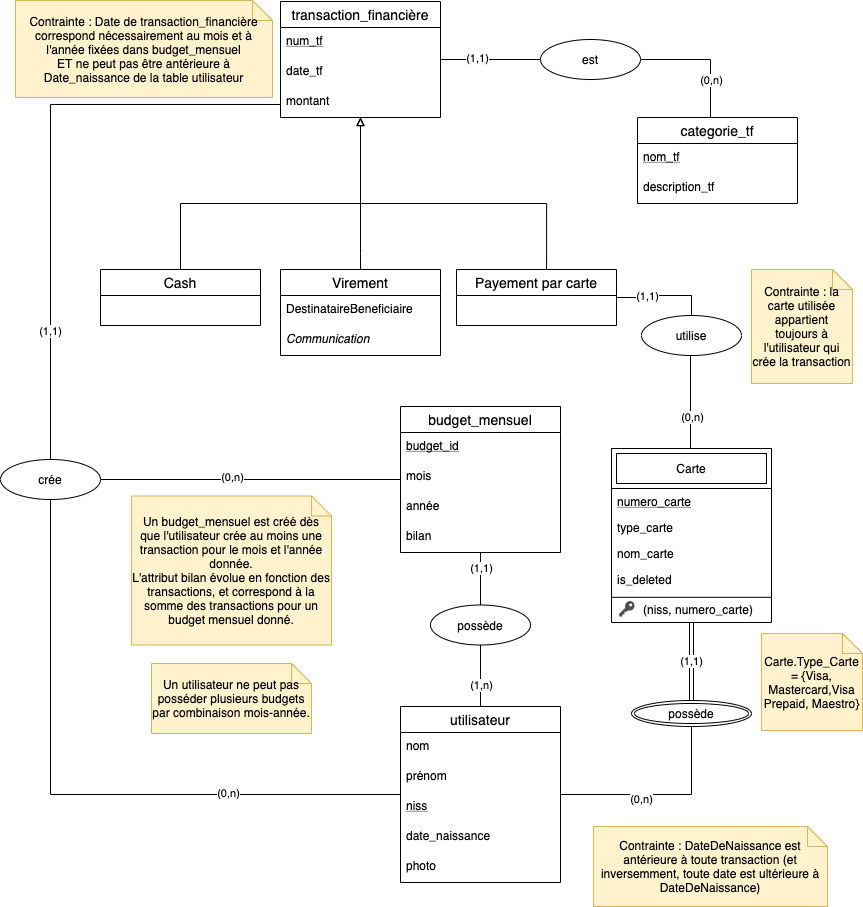
\includegraphics[scale=0.6]{schema_ea_final_v2.png}}
\caption{\footnotesize{Schéma conceptuel entité-association de la base de données exploitée par Budget Squirrel}}
\end{figure}

\newpage 

\section{Schéma logique relationnel}

Vous trouverez ci-dessous notre traduction du schéma entité association présenté à la section précédente, ainsi que les contraintes supplémentaires, et quelques explications de traduction.

\begin{Verbatim}[commandchars=+\[\]]
utilisateur(nom, prenom, +underline[niss], date_naissance, photo)
	utilisateur.niss = {froggy.png, gollum.jpg, politecat.jpg, raccoon.jpg}

carte(nom_carte, +underline[numero_carte], type_carte, +underline[niss_util], is_deleted)
	carte.niss_util référence utilisateur.niss
	carte.type_Carte = {Visa, Mastercard,Visa Prepaid, Maestro}

budget_mensuel(+underline[budget_id], mois, annee, bilan, niss_util) 
	budget_mensuel.niss_util référence utilisateur.niss

transaction_financiere(+underline[num_tf], date_tf, montant, budget_id, niss_util, cat_tf)
	transaction_financiere.budget_id référence budget_mensuel.budget_id
	transaction_financiere.cat_tf référence categorie_tf.nom_tf
	transaction_fianciere.niss_util référence utilisateur.niss

tf_cash(+underline[num_tf])
	tfcash.num_tf référence transaction_financiere.num_tf

tf_virement(+underline[num_tf], destbenef, +it[communication])
	tfvirement.num_tf référence transaction_financiere.num_tf

tf_carte(+underline[num_tf], +underline[numero_carte])
	tf_carte.num_tf référence transaction_financiere.num_tf	
	numero_carte référence carte.numero_carte

categorie_tf(+underline[nom_tf], description_tf)
\end{Verbatim}

Contraintes définies :

\begin{itemize}
\item utilisateur.niss ne peut contenir que 11 caractères, spécifiquement 11 chiffres, pas plus, ni moins;
\item La valeur par défaut de carte.is\_deleted est 0 (zéro);
\item La valeur de carte.numero\_carte contient uniquement des chiffres, et ne peut contenir que 16 ou 17 chiffres;
\item budget\_mensuel.budget\_id correspond a une combinaison unique de niss\_util, mois et année, ainsi, il est impossible pour un même utilisateur de posséder plusieurs budgets pour le même mois et la même année;
\item budget\_mensuel.bilan correspond à la somme de toutes les transactions pour un utilisateur, un mois et une année données;
\item transaction\_financiere.date\_tf (et par extension, le mois et l'année de budget\_ mensuel) sont nécessairement ultérieures à utilisateur.date\_naissance;
\item transaction\_financiere.budget\_id ne peut référencer qu'un budget\_id dont le mois et l'année correspondent à transaction\_ financiere.date\_ tf;
\item Dans la table tf\_carte, transaction\_financière.num\_tf et carte.numero\_carte référencent obligatoirement le même niss\_util : un utilisateur ne peut qu'utiliser les cartes qui lui sont liées pour les transaction qui lui sont liées;
\item transaction\_financière.num\_tf doit se retrouver une et une seule fois soit dans la table tf\_carte, soit dans la table tf\_virement, soit dans la table tf\_cash;
\item \textbf{Autres?}
\end{itemize}

L'héritage entre la table transaction\_financière et les tables cash, virement, et payement par carte a été traduit par une matérialisation, que nous représentons graphiquement à la figure \ref{materialisation}.
Nous avons choisi d'utiliser la matérialisation afin de conserver la super-entité, ainsi que les sous-entités, et la relation sémantique qu'elles entretiennent.
La relation est considérée comme totale et exclusive : une transaction financière est au moins une transaction en liquide, par virement ou payée par carte, mais ne peut pas être de plus d'un type à la fois.
L'association un à plusieurs entre utilisateur et budget\_mensuel a été traduite en plaçant la référence du côté "un" de l'association : ainsi, on retrouve utilisateur.niss dans budget\_mensuel.niss\_util.
Il en est de même pour la table transaction\_financière, à laquelle nous avons ajouté une référence et au budget\_mensuel, et au NISS de l'utilisateur.
Toujours en suivant la même logique, l'entité faible carte contient son attribut identifiant lié au NISS de l'utilisateur, et la clé de la table est formée de la combinaison NISS - numéro de carte.

\begin{figure}[!ht]
\noindent
\makebox[\textwidth][c]{
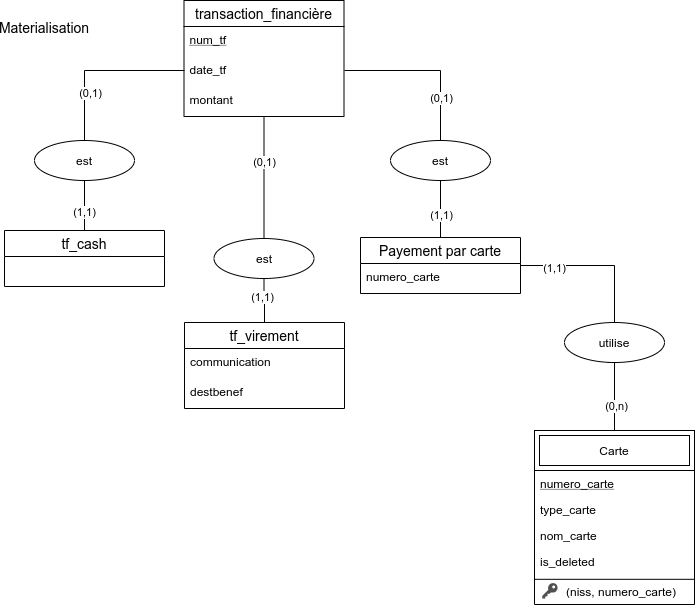
\includegraphics[scale=0.5]{materialisation.png}}
\caption{\footnotesize{Matérialisation de l'héritage entre les transactions}}
\label{materialisation}
\end{figure}

\newpage

\section{Code SQL}

\subsection{Description du code de création de la base de données}

Description du code sql de création de la db 
!! La création de la db doit : créer des tables , avoir des contraintes de clé primaire, unique et externe, avoir des contraintes sous forme de prédicat de table et de colonne, avoir des procédures stockées et des déclencheurs

\subsection{Éléments de SQL avancé}

\subsubsection{Contraintes garanties par des check}

\subsubsection{Requêtes de consultation}

\subsubsection{Requêtes de mise à jour}


\subsubsection{Vues utilisées}

La base des données contient quatre vues qui sont utilisées dans la construction d'historiques et des statistiques dans l'application : 

\begin{enumerate}
\item historique\textunderscore v, qui liste chronologiquement les informations liés aux transactions effectuées par un utilisateur,
\item stat\textunderscore depenses\textunderscore revenus\textunderscore mois, qui liste chronologiquement les dépenses et les revenus enregistrés par l'utilisateur, en faisant également le bilan des dépenses, le bilan des revenus, et le bilan total,
\item stat\textunderscore cat, qui liste la répartition totale des dépenses et des revenus par catégorie et par utilisateur, 
\item et stat\textunderscore types, qui liste la répartition du budget global par type de transaction employé dans le payement, ainsi que par nombre d'emplois de chaque type de transaction, pour un bilan global des dépenses et revenus.
\end{enumerate}

Ces vues sont utiles à la gestion et à l’agrégation des données, et permettent notamment d'offrir à l'utilisateur de l'application différents graphiques et informations agrégées sur son budget.

Ce qu'on utilise pour l'historique et les différentes statistiques

\subsubsection{Déclencheurs}


\subsubsection{Droits d'accès}

\newpage
\section{Description de l'application Web}

L'application web que nous avons développé a pour objectif de permettre aux utilisateurs de s'inscrire, d'enregistrer leurs transactions, de consulter leur historique par mois, ainsi que des statistiques sur la répartition de leurs dépenses, de leur revenus, et un bilan total de leur budget. 
L'accès à la base de données est restreint : ce n'est pas un accès root, mais bien un accès spécifiquement défini pour les utilisateurs de l'application. Nous en avions fait la description détaillée à la section précédente.

À l'ouverture de l'application (\verb\localhost/budgetsquirrel/index.html\ ou simplement \verb\localhost/budgetsquirrel/\), l'utilisateur a deux possibilités : se connecter, ou s'inscrire.

\begin{figure}[!ht]
\noindent
\makebox[\textwidth][c]{
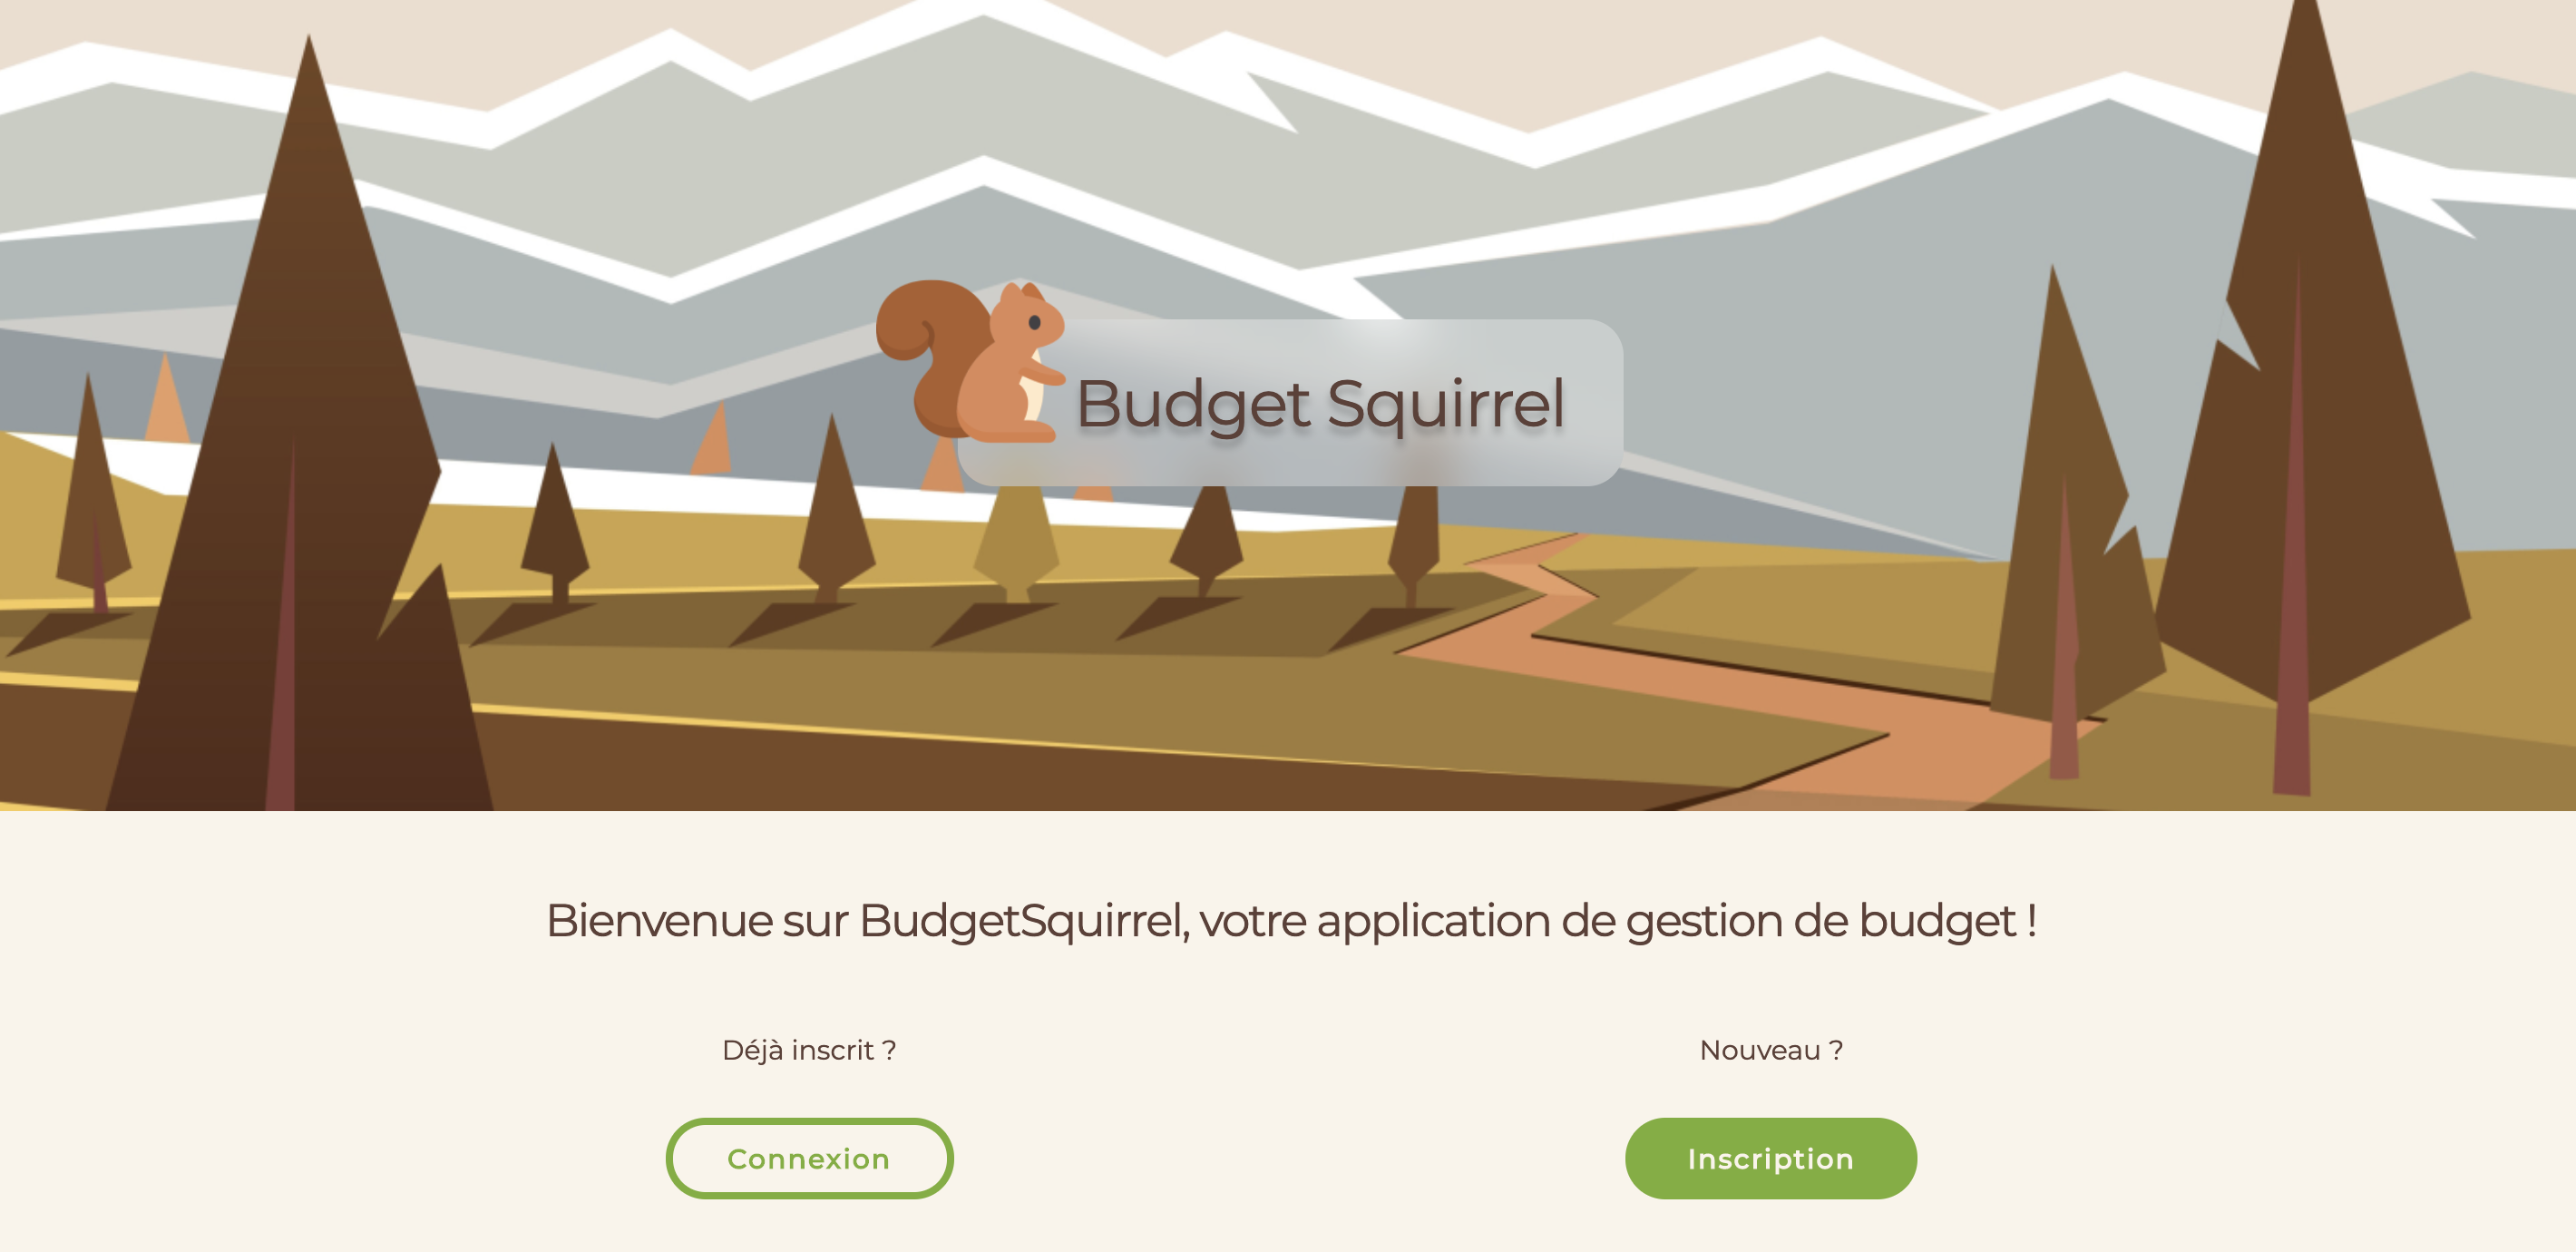
\includegraphics[scale=0.25]{index.png}}
\caption{\footnotesize{Landing page pour Budget Squirrel}}
\end{figure}

S'il choisit de s'inscrire, il est redirigé vers un formulaire d'inscription où il doit rentrer son nom, son prénom, son NISS, et choisir une photo de profil. 

\begin{figure}[!ht]
\noindent
\makebox[\textwidth][c]{
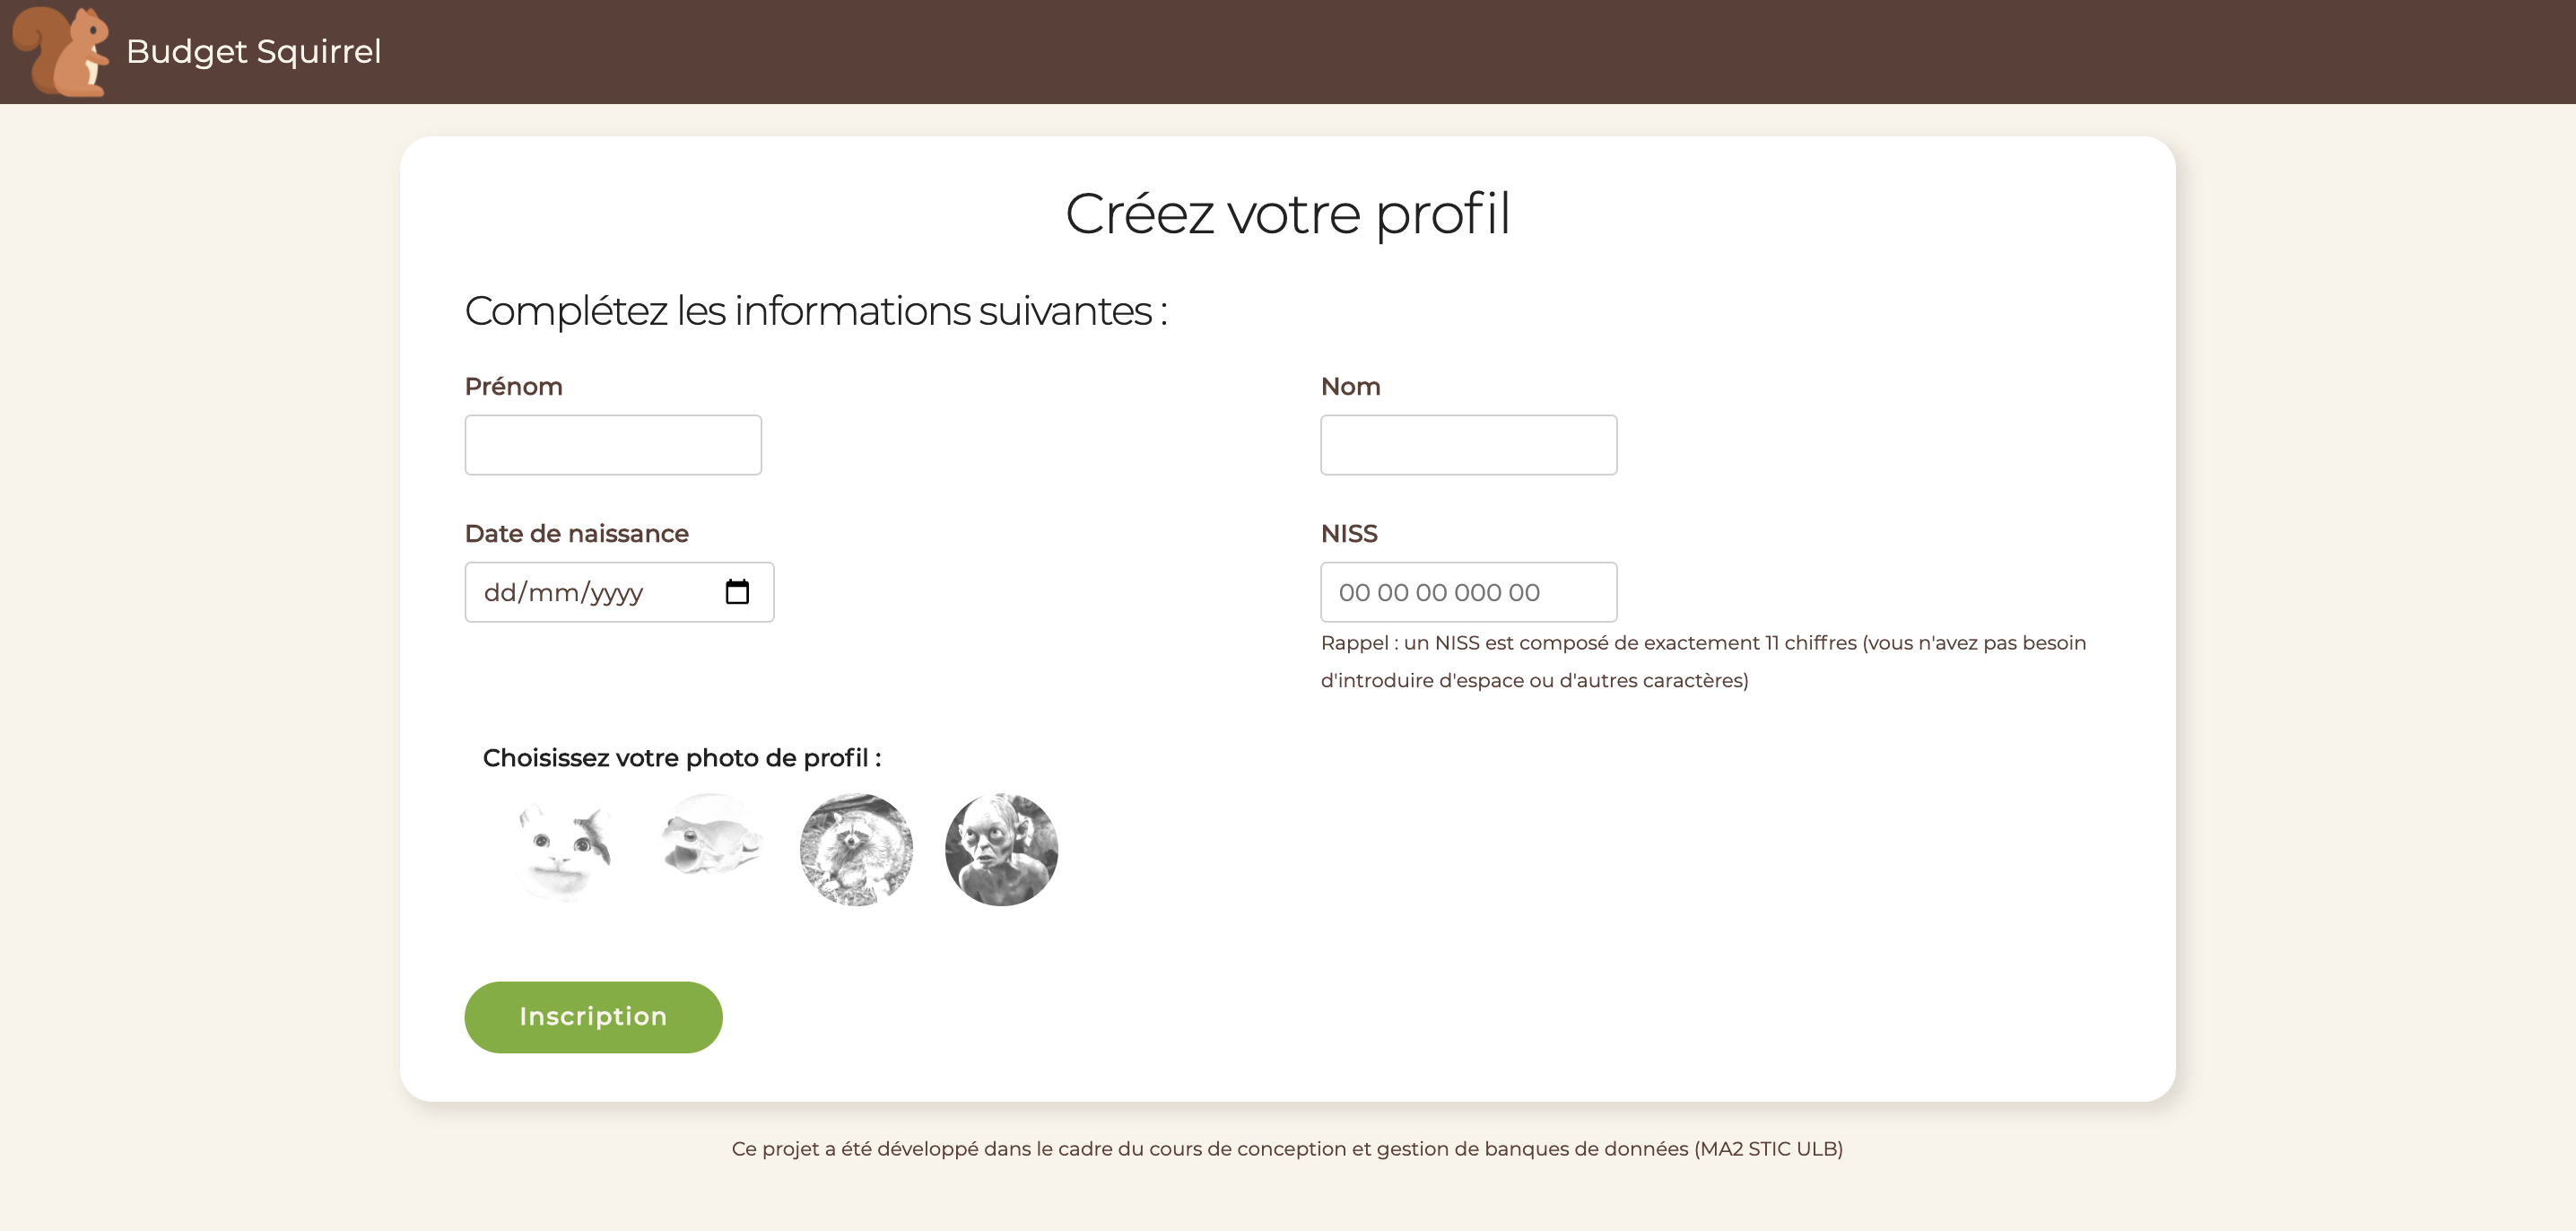
\includegraphics[scale=0.25]{inscription.png}}
\caption{\footnotesize{Écran inscription Budget Squirrel}}
\end{figure}

Si un utilisateur est déjà inscrit sous le NISS entré, il en est notifié (et a la possibilité de se rediriger vers la page de connexion). Si le NISS n'est pas encore utilisé par un utilisateur, l'enregistrement se fait, l'utilisateur est notifié du succès de ce dernier, et peut se rediriger vers la page de connexion. La vérification de la présence d'un utilisateur utilisant déjà le NISS se fait à deux niveaux : au niveau de la base de données en elle-même, comme nous l'avons vu au dessus, grâce à la contrainte de clé primaire, et également en PHP, en faisant une sélection de la table utilisateur (si la sélection par rapport au niss entrée renvoie un résultat différent de zéro, l'utilisateur est notifié de l'impossibilité de créer un compte avec ce NISS).

La page de connexion, par souci de simplification, est une simple sélection de profil : l'utilisateur a accès à la liste des utilisateurs, sélectionne son profil (nom et prénom) dans la liste , et se connecte. Ensuite, le NISS de l'utilisateur est récupéré par une méthode POST, enregistré par la méthode SESSION et appelé grâce à \verb\session_start();\ à chaque page de l'application où il est enregistré comme connecté).

\begin{figure}[!ht]
\noindent
\makebox[\textwidth][c]{
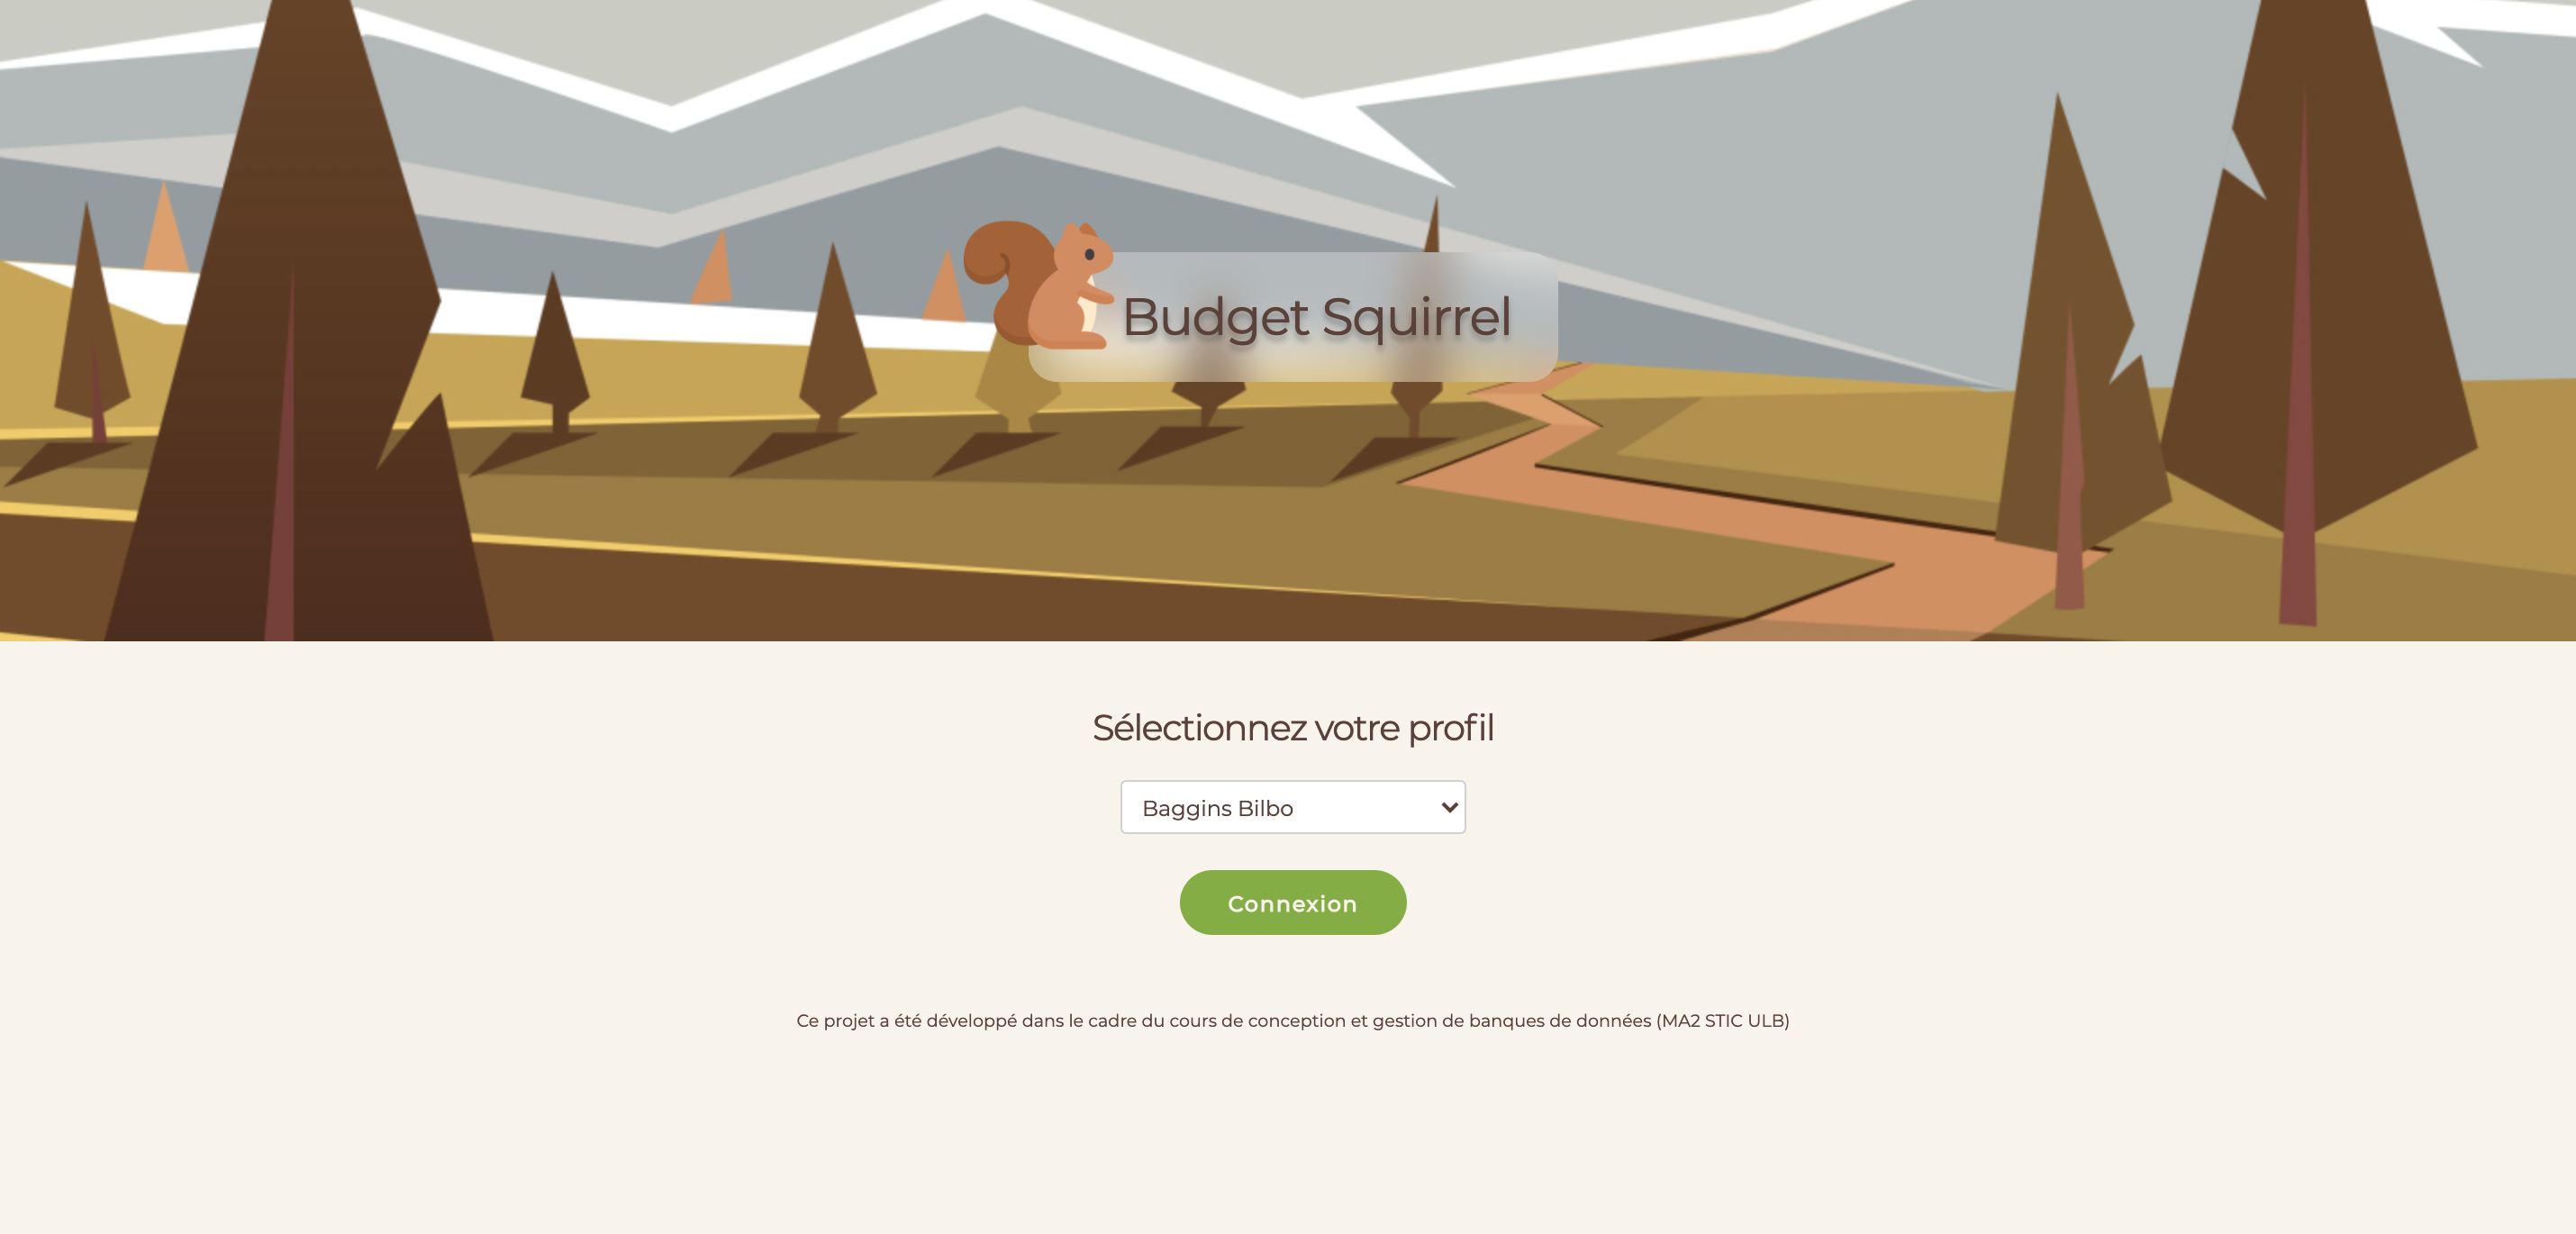
\includegraphics[scale=0.3]{connexion.png}}
\caption{\footnotesize{Écran connexion Budget Squirrel}}
\end{figure}

Une fois qu'il a sélectionné son profil et choisi de se connecter, l'utilisateur est redirigé vers une page d'accueil. La page d'accueil présente brièvement les différentes pages de l'application. Depuis la barre de navigation, présente sur toutes les pages (sauf celles ou l'utilisateur n'est pas considéré comme connecté), l'utilisateur a accès : à la page d'accueil, à l'historique, à la page d'enregistrement, à la page de statistiques, et à sa page personnelle de profil. Il peut ainsi naviguer librement entre les différentes pages.

\newpage
\begin{figure}[!ht]
\noindent
\makebox[\textwidth][c]{
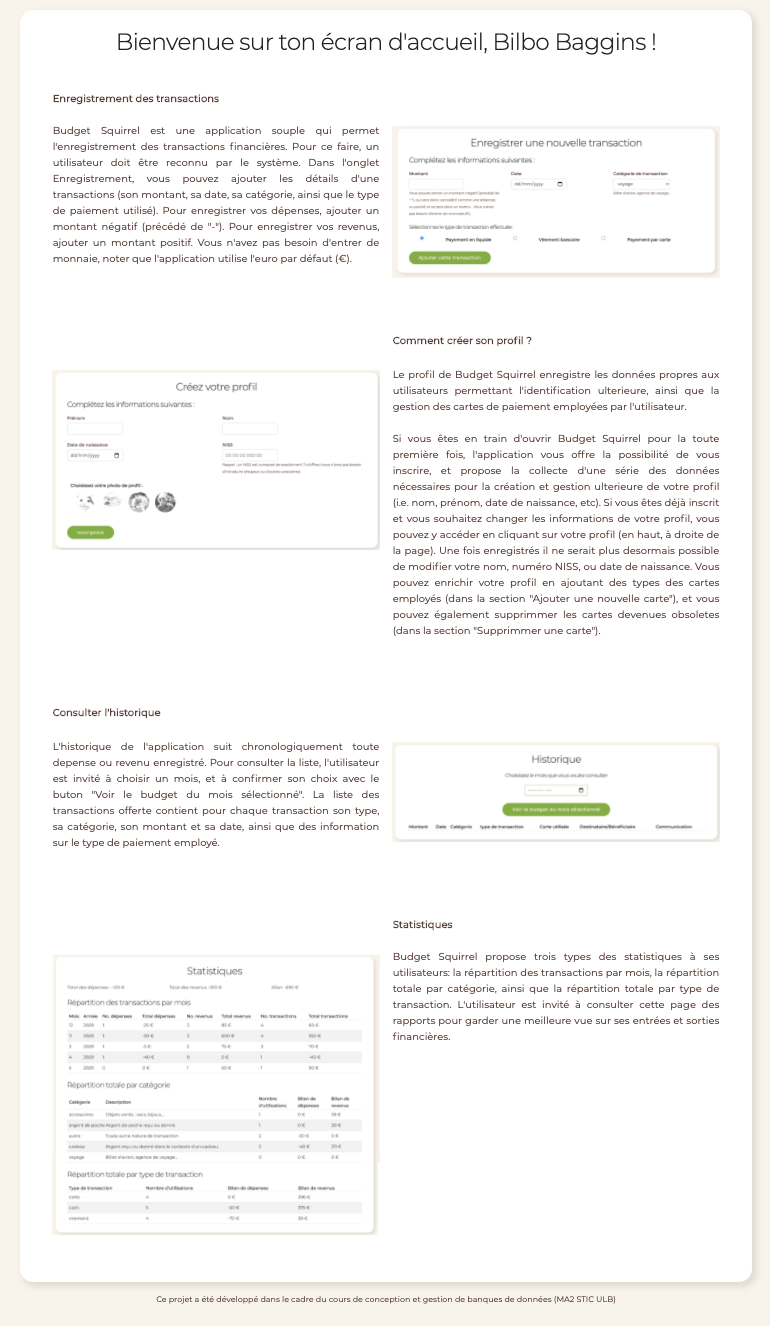
\includegraphics[scale=0.90]{homepage.png}}
\caption{\footnotesize{Page d'accueil Budget Squirrel}}
\end{figure}

\newpage
La page personnelle de profil permet à l'utilisateur de visualiser ses informations : nom, prénom, NISS, date de naissance. Il peut également y ajouter et y supprimer ses cartes\footnote{Cette suppression est une suppression logique du côté de la base de données : les cartes possèdent une colonne is\_deleted , par défaut la valeur de la colonne est à 0, et si l'utilisateur \og supprime\fg sa carte, la valeur passe à 1, et la carte est considérée comme virtuellement supprimée} . Les listes de ses cartes disponibles et de ses anciennes cartes sont également visibles depuis la page de profil. Il peut également y actualiser sa photo.

\begin{figure}[!ht]
\noindent
\makebox[\textwidth][c]{
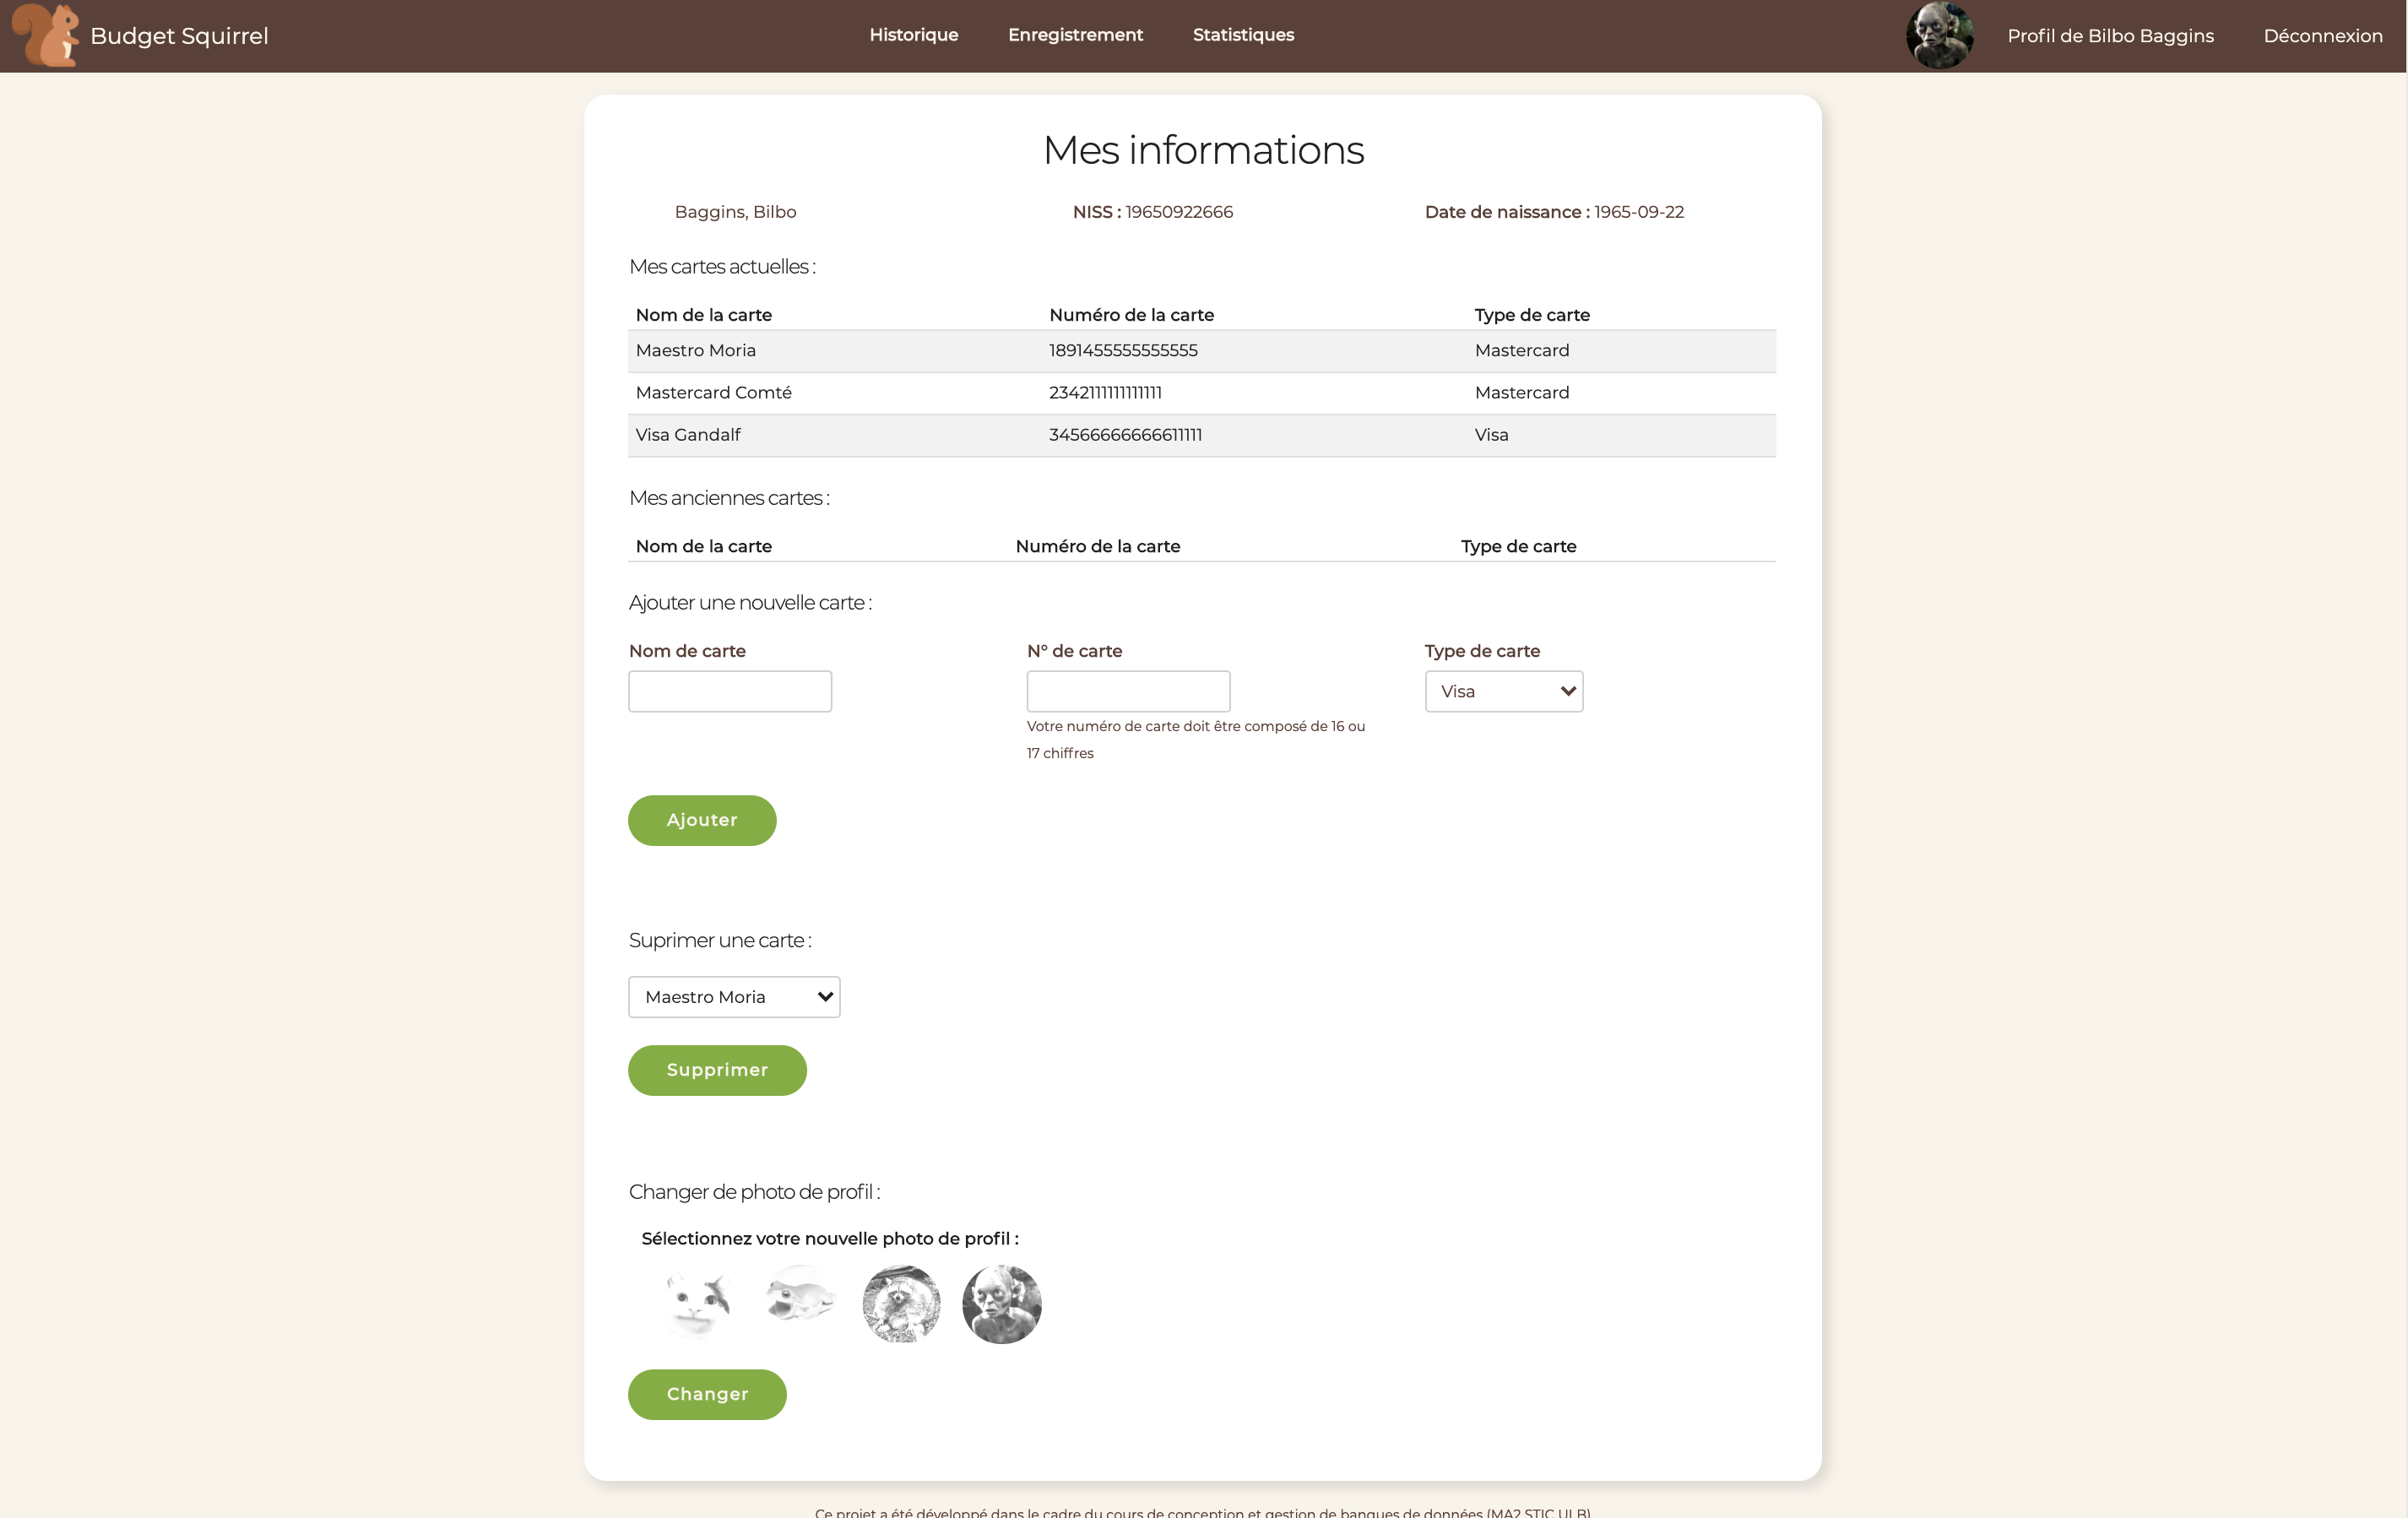
\includegraphics[scale=0.25]{profil.png}}
\caption{\footnotesize{Page personnelle Budget Squirrel}}
\end{figure}

La page d'enregistrement permet d'enregistrer des transactions. L'utilisateur est obligé d'entrer un montant, de sélectionner une date, une catégorie de transaction, et un type de transaction (à nouveau, la vérification se fait une fois en PHP, et une fois aussi du côté de la base de données). En fonction du type de transaction effectuée, il doit également ajouter des informations supplémentaires. Le payement en liquide ne demande aucune information supplémentaire, le virement bancaire demande d'introduire un destinataire ou un bénéficiaire, et éventuellement une communication, et un payement par carte nécessite de sélectionner la carte utilisée. Cet aspect est géré uniquement en PHP, et demande donc de faire deux opérations consécutives si l'on veut rentrer le type de transaction sans passer par l'application Web.

\begin{figure}[!ht]
\noindent
\makebox[\textwidth][c]{
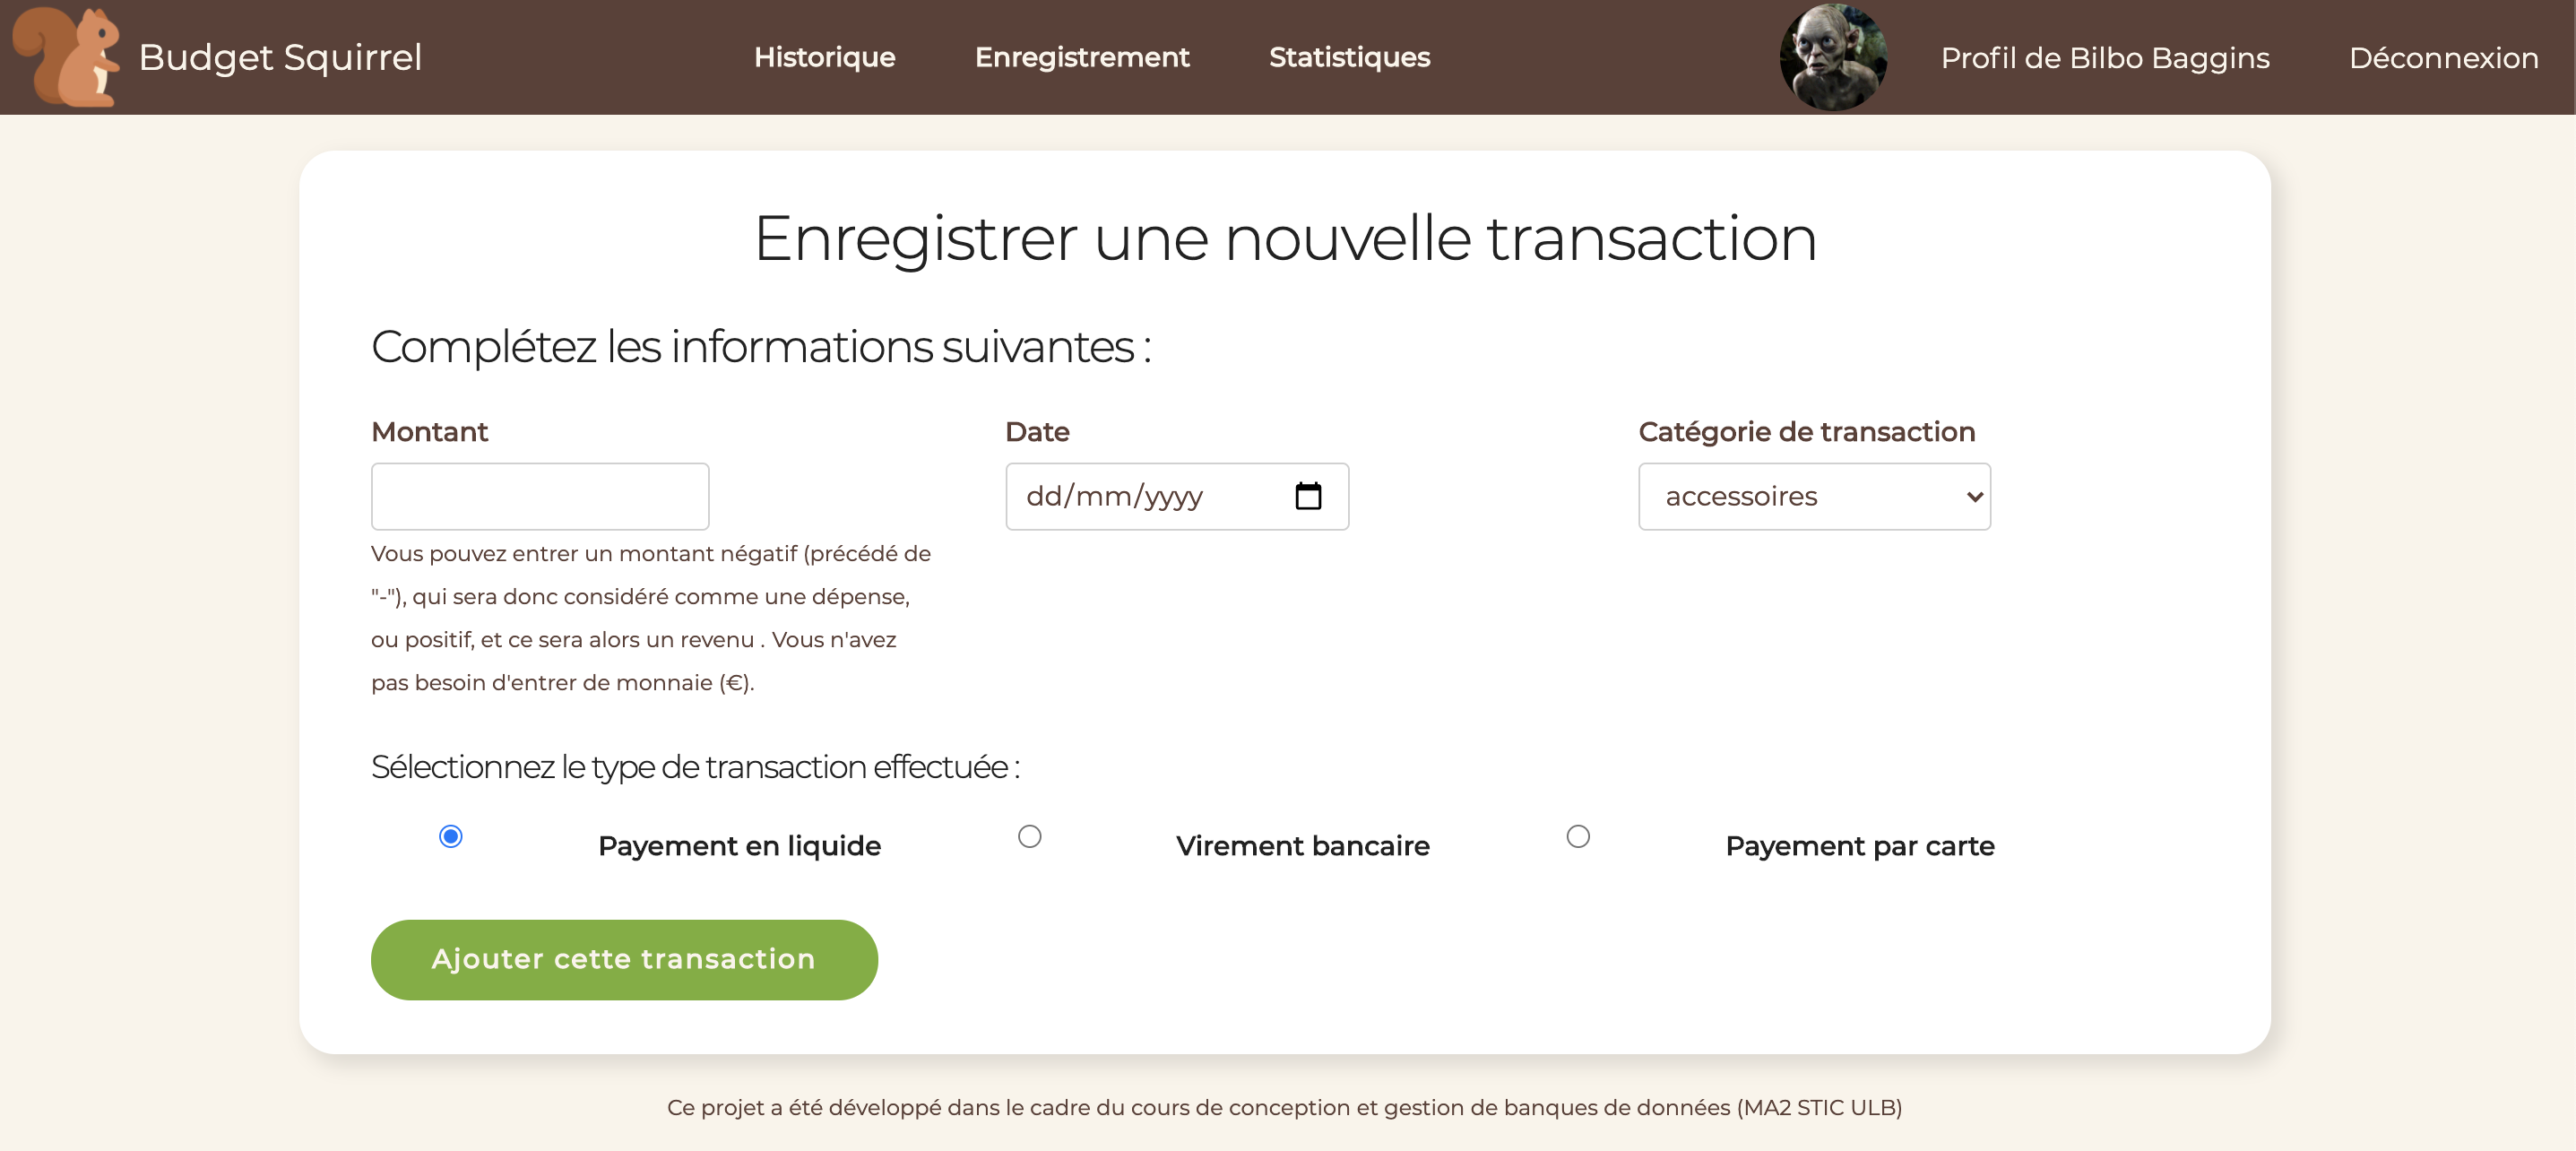
\includegraphics[scale=0.25]{enregistrement.png}}
\caption{\footnotesize{Enregistrement des transactions en Budget Squirrel}}
\end{figure}

\newpage
La page historique permet à l'utilisateur de visualiser les transactions effectuées : pour cela, il doit d'abord sélectionner le mois et l'année dont il veut consulter le budget. Il a alors accès à un tableau affichant le montant, la date, la catégorie, et le type de transaction effectuée, et éventuellement la carte utilisée, le destinataire/bénéficiaire, et la communication. En dessous de la table, l'utilisateur peut également voir le bilan total du mois. Enfin, il peut également choisir de supprimer une des transactions affichées.

\begin{figure}[!ht]
\noindent
\makebox[\textwidth][c]{
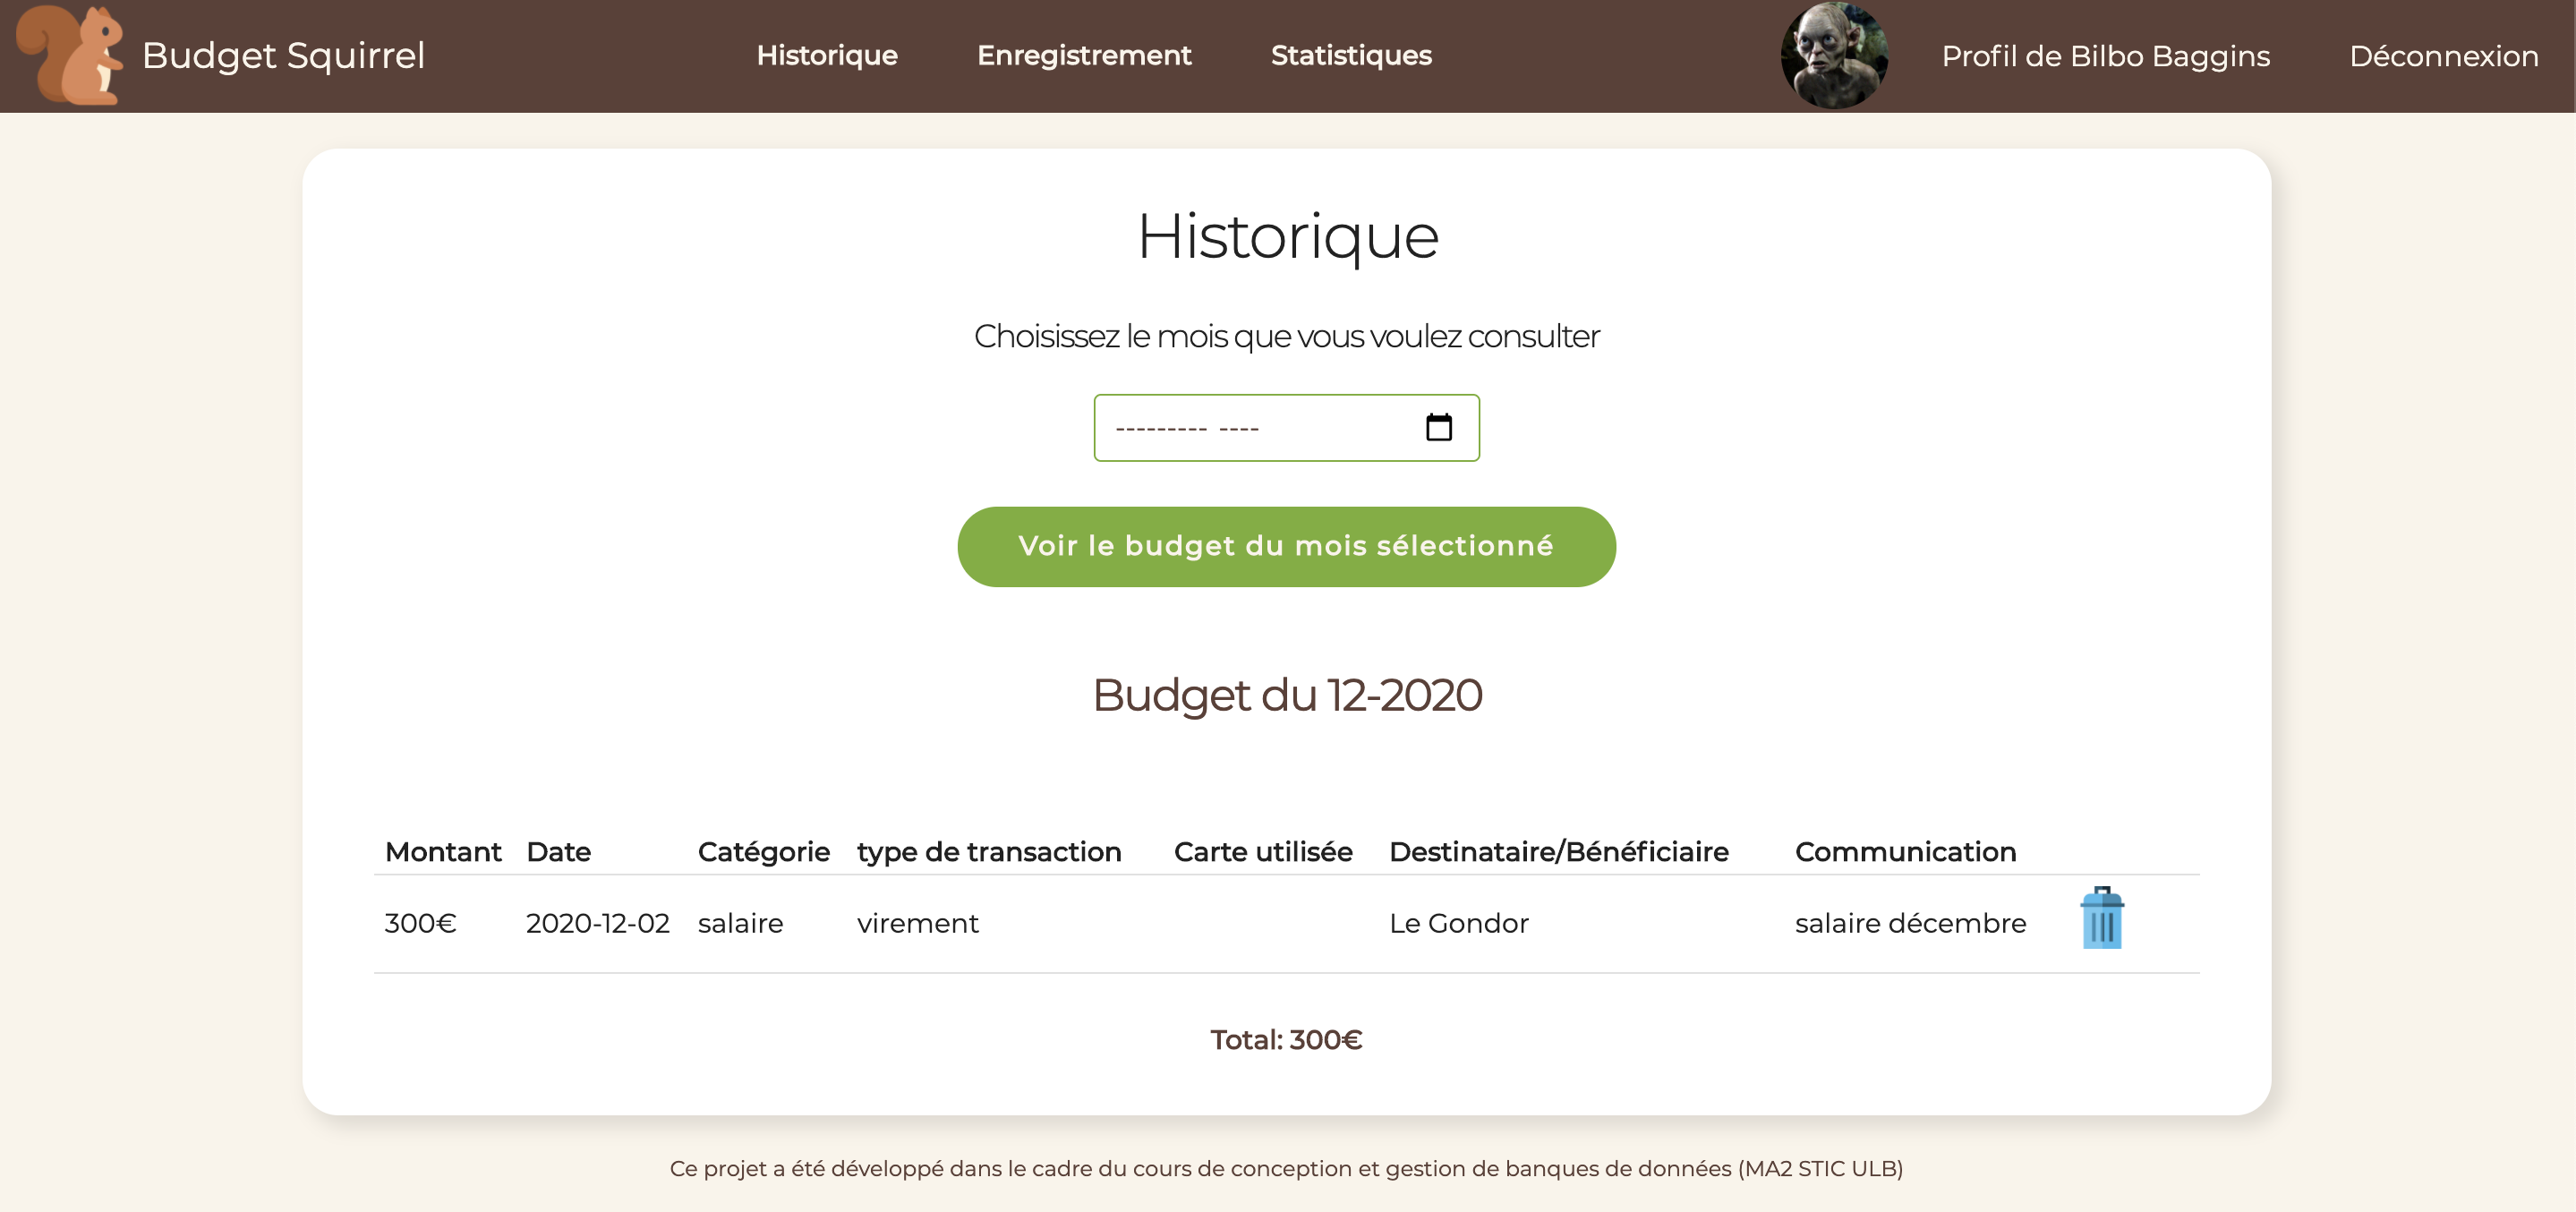
\includegraphics[scale=0.25]{historique.png}}
\caption{\footnotesize{Historique des transactions en Budget Squirrel}}
\end{figure}

L'écran de statistiques offre différentes informations sur les données concernant l'utilisateur. Les informations offertes sont les suivantes : un total des dépenses, un total des revenus, et un bilan, mais aussi un tableau montrant la répartition des transactions (dépenses et revenus) par mois, ainsi que le bilan par mois, pour une vue plus condensée de l'historique, un tableau montrant la répartition totale par catégorie (couplé à une description de chaque catégorie), et  enfin la répartition des transactions entre les différents types de payements (le nombre d'utilisations, le bilan des dépenses et le bilan des revenus pour chaque type de transaction).

À tout moment, l'utilisateur peut également se déconnecter, en cliquant, en haut à droite de la barre de navigation, sur "déconnexion". Les informations de sessions (donc, le NISS sous lequel l'utilisateur est connecté) sont effacées, et l'utilisateur peut choisir de retourner à l'écran d'accueil.

\begin{figure}[!ht]
\noindent
\makebox[\textwidth][c]{
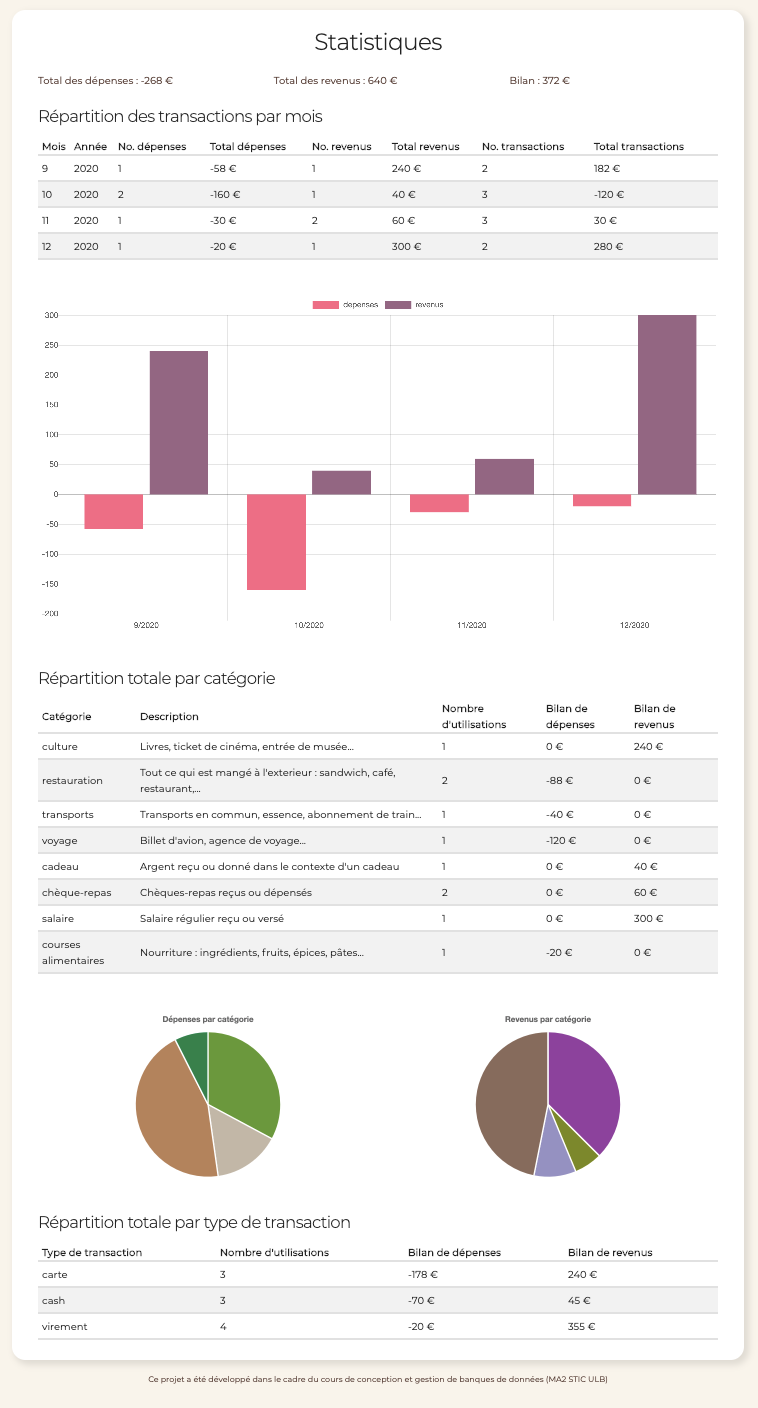
\includegraphics[scale=0.7]{stat.png}}
\caption{\footnotesize{Statistiques Budget Squirrel}}
\end{figure}

\newpage

\section{Développement du projet}

Budget Squirrel est une application consistante d'une base des données et une interface client. Le design, développement et administration d'une telle application nécessitent donc une chorégraphie particulière, reposant sur des livrables qui doivent être prêts à l'emploi dans une certaine séquence, et qui se trouvent la plupart de temps dans une symbiose étroite. De plus, certaines exigences du projet, établies ou agréées dès le départ, et révisés pendant les séances d'entretien projet, ainsi que certaines contraintes liées à d'autres engagements impératives pour les développeurs se sont vite imposées comme des conditions demandaient une coordination ainsi qu'une communication ouverte et souple au sein du groupe. Le groupe s'est vite mis d'accord sur une division des tâches qui prend en compte les contraintes relatives aux disponibilités de chacune d'entre nous, ainsi qu'aux préférences des techniques et outils des développement, toute en gardant en vue l'impératif d'avoir touché au moins une fois à chaque écran et surtout d'avoir participé en tandem le plus que possible dans les parties couvrant la matière vue au cours.

\subsection{Travail conceptuel et outils employés pour démarrer le projet}

En suivant le calendrier communiqué au cours, le groupe à fait sa proposition de projet le 3 octobre, et a reçu une confirmation pour le deuxième sujet dans un bref délai.

\begin{figure}[!ht]
\noindent
\makebox[\textwidth][c]{
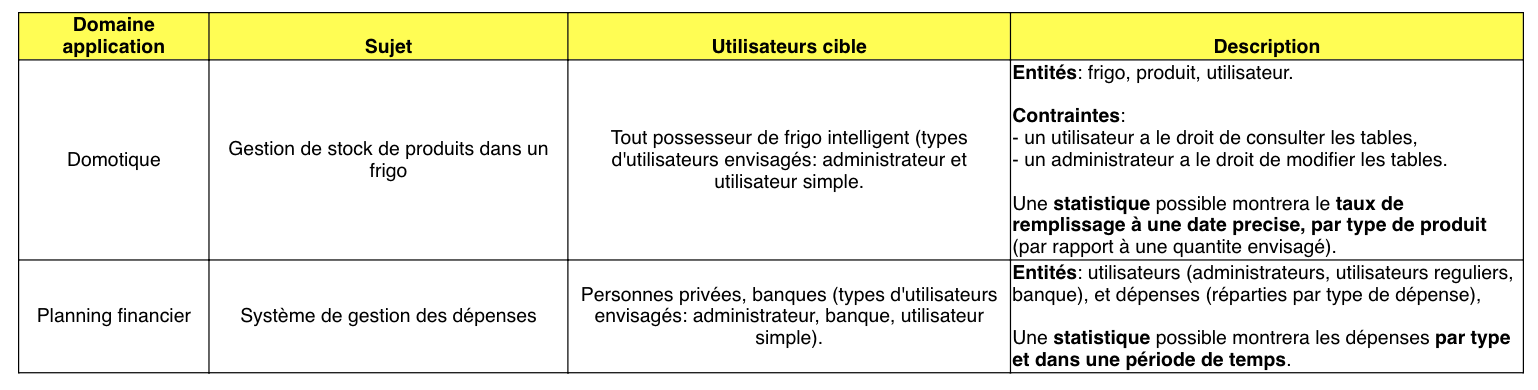
\includegraphics[scale=0.56]{proposal.png}}
\caption{\footnotesize{Sujets proposés en vue de développement}}
\end{figure}

Une fois le choix de projet validé, nous avons commencé le travail de conceptualisation, avec un double-but: la conception d'un modèle entité-association, ainsi qu'une première ébauche d'interface client. Pour nous aider dans le démarche EA, nous avons employé l'application web draw.io, et en ce qui concerne l'interface client, l'outil Figma à été employé dans la construction des wireframes. Le résultat de ce travail s'est matérialisé dans un rapport préliminaire, présenté pour évaluation et validation le 31 octobre. C'est en suivant ce rapport préliminaire  que nous avons par la suite développé les éléments décrits dans les sections 2 et 3 du présent rapport.
 
\subsection{Design et techniques de travail }

La partie design à été facilité par l'emploi d'une structure html ouverte, que nous avons taillé aux besoins de notre application. Cette étape à rajouté une première couche de complexité en ce qui concerne l'imbrication des langages utilisés, en ajoutant PHP et HTML aux requêtes SQL. Le PHP étant un langage très flexible, il nous a été relativement facile de créer de nombreuses contraintes, et de combiner différentes requêtes SQL pour que l'application réponde exactement comme il faut à tout input de l'utilisateur. 
Par contre, un des défis que nous avons rencontré durant le développement de ce projet a été l'écriture de données en utilisant du SQL pur, sans l'aide de l'application. Certains éléments, facilement mis en place en PHP, étaient difficiles à traduire en SQL.
Une deuxième couche de complexité à été rajouté par l'introduction des éléments javascript de visualisation dynamique des données (toggle screen, et graphes dynamiques) et des éléments en SQL d'aggregation des données (vues statistiques). De façon général, une des parties la plus difficile à été d'orchestrer, d'une façon robuste et cohérente, la partie d'insertions, mises à jour, et suppressions, afin d'éviter la perte des données, ou bien le double encodage. Faire le choix entre l'ajout des contraintes au niveau de client, ou bien au niveau de la base des données, ainsi que naviguer les contraintes implémentés, n'était pas toujours facile. Pour parer ces difficultés nous avons employé la technique de programmation en binôme (asynchrone, en utilisant GitHub pour partager les mises à jours au niveau du code, et Teams pour faciliter la communication). La taille restreinte du groupe à particulièrement facilité ce méthode de travail, et nous à permis une prise de décision rapide.
La section 5 du rapport témoigne sur les choix qui ont été gardés et implémentés au niveau de design d'application.

\subsection{Quelques scénarios de test }

\textbf{Nécessaire?}

\newpage
\section{Conclusion}

\subsection{Défis et solutions}
\subsection{Limites et possibilités de développement}
Les points forts et faiblesses d’application, le temps nécessaire pour développer le concept avec deux personnes, les sources consultées pour la partie pratique (i.e. les slides, ou techniques vues au TP, ainsi que les conseils d’assistante, mais aussi w3schools ou bien stackoverflow).
Finalement quelques mots sur l'expérience du projet.

Améliorations : 
- vérification du niss par rapport à la date de naissance de l'utilisateur
- finalement, le bilan dans la table budget mensuel n'est pas obligatoire
- choix de la matérialisation pour la traduction de l'héritage : remise en question




\newpage

%voir si bibliographie nécessaire
%\chapter*{Bibliographie} 
%\addcontentsline{toc}{chapter}{Bibliographie}
%\markboth{Bibliographie}{}
%
%\printbibliography[heading=none]
%
%\fussy

%Voir si annexes nécessaire
%\chapter*{Annexes}
%\addcontentsline{toc}{chapter}{Annexes}
%\markboth{Annexes}{}

\end{document} % fin du corps du texte